\chapter{Идеальный ферми--газ}
Идеальный Ферми-газ (далее ИФГ) -- это система невзаимодействующих фермионов (частиц, имеющих полуцелый спин).
Согласно принципу запрета Паули \cite{Pauli:ZP:1925,Pauli:PR:1940}, в заданном квантовом состоянии может находиться только один фермион.
Это приводит приводит к нескольким следствиям.
Во-первых, полная энергия ИФГ при нулевой температуре отлична от нуля.
Во-вторых, давление ИФГ не равно нулю при нулевой температуре, в отличие от идеального больмановского газа.

В дальнейшей части работы используется атомная система единиц, в которой редуцированная постоянная Планка, масса и заряд фермиона равны единице.
Помимо этого, постоянная Больцмана тоже положена равной единице.

\section{Химический потенциал и его производные}
Для системы фермионов распределение частиц по энергиям задается статистикой Ферми-Дирака \cite{Landau:statmech:1958}:
\begin{equation}
    n_k = \frac{1}{\exp{[(\varepsilon_k - \mu)/T]} + 1}.
    \label{eq:fd}
\end{equation}
Здесь $\mu$ есть химический потенциал, $T$ -- температура системы, а $\epsilon_k$ -- энергия $k$-ого квантового состояния. 
Полное число частиц получается суммированием \eqref{eq:fd} по всем возможным значениям энергии.
Полагая $\epsilon_k = p^2_{k} / (2m)$ и переходя к квазинепрерывному спектру по $k$, после сведения к интегрированию по энергии получим:
\begin{equation}
    \label{eq:conc}
    \frac{N}{V}=\frac{g}{\sqrt{2} \pi^{2}} \int_{0}^{\infty} \frac{\sqrt{\varepsilon} d \varepsilon}{e^{(\varepsilon-\mu) / T}+1}.
\end{equation}
Здесь $V$ -- объем системы.
Вводя безразмерный $y = \mu / T$ и объем на одну частицу $v = V / N$, можно переписать \eqref{eq:conc} в следующем виде:
\begin{equation}
    \frac{1}{v} = \frac{g T^{3/2}}{\sqrt{2}\pi^2}I_{1/2}(y).
    \label{eq:mu_equation}
\end{equation}
Здесь введен т.н. интеграл Ферми-Дирака:
\begin{equation}
    \label{eq:fermi-dirak_integral_definition}
    I_{j}(y)= \int_{0}^{\infty} \frac{t^{j}}{e^{t-y}+1} dt
\end{equation}
\begin{equation}
    \label{eq:ifg_diff_rule}
    \frac{d}{dx}\, I_k (x) = k I _{k-1} (x)
\end{equation}

Уравнение \eqref{eq:mu_equation} задает химический потенциал как функцию от температуры и удельного объема: $\mu = \mu(v, T)$.
В секциях \ref{sec:asymp_low}, \ref{sec:asymp_high} приводится его решение в различных температурных пределах.

В дальнейшем нам понадобятся первые и вторые производные $\mu(v, T)$.
Для их получения продифференцируем \eqref{eq:mu_equation} по соответствующим переменным с учетом свойства \eqref{eq:ifg_diff_rule} и разрешим получающиеся уравнения относительно производных. Это даст следующие результаты:
\begin{equation}
   \label{eq:mu_T}
   y'_{T} = -\frac{3 I_{1 / 2}(y)}{T I_{-1 / 2}(y)}
\end{equation}

\begin{equation}
   \label{eq:mu_v}
   y'_{v} = - \frac{2 I_{1 / 2} (y)}{v I_{-1 / 2} (y)}\,
\end{equation}

\begin{equation}
   \label{eq:mu_vv}
   y''_{vv} = \frac{4 I_{1 / 2} (y)}{v^2 I_{-1 / 2} (y)}\, + \frac{2 I_{-3 /2} (y) I_{1 / 2} ^2 (y)}{v^2 I_{-1 /2}^3 (y)}\,
\end{equation}

\begin{equation}
   \label{eq:mu_TT}
   y''_{TT} = \frac{15 I_{1 /2} (y)}{2 T^2 I_{-1 /2} (y)}\, + \frac{9 I_{-3 /2}(y) I_{1 /2}^2 (y)}{2 T^2 I_{-1 /2}^3 (y)}\,
\end{equation}

\begin{equation}
   \label{eq:mu_vT}
   y''_{vT} = y''_{Tv} = \frac{3 I_{1 /2}(y)}{T v I_{-1 /2} (y)}\, + \frac{3 I_{-3 /2} (y) I_{1 /2}^2 (y)}{T v I_{-1 /2}^3 (y)}\,
\end{equation}

\section{Термодинамические функции ИФГ}
Согласно \cite{kirzhnits:UFN:1975}, выражение для свободной энергии Гельмгольца имеет вид:
\begin{equation}
   \label{eq:helmholtz_potential}
   F = \frac{g}{\sqrt{2}\pi^2}\,  T^{5 / 2} v \left( y \, I_{1 /2} (y) - \frac{2}{3}\, I_{3 / 2} (y) \right)
   = T\left[y - \frac{2}{3}\frac{I_{3/2}(y)}{I_{1/2}(y)}\right].
\end{equation}
Последнее равенство получается подстановкой $v$ из \eqref{eq:mu_equation}.
Из выражения для $F$ можно получить остальные термодинамические величины:
\begin{equation}
    \label{eq:PES}
    P = -F'_v;\quad
    E = F - TF'_T;\quad
    S = -F'_T;
\end{equation}
\begin{equation}
    \label{eq:CVCP}
    C_V = -TF''_{TT};\quad
    C_P = -TF''_{TT} + \frac{T(F''_{vT})^2}{F''_{vv}};
\end{equation}
\begin{equation}
    \label{eq:CTCS}
    C_T^2 = v^2F''_{vv};\quad
    C_S^2 = v^2F''_{vv} - \frac{v^2(F''_{vT})^2}{F''_{TT}};\quad
    \gamma = \frac{VF''_{vT}}{TF''_{TT}};\ \ldots
\end{equation}
Здесь $P$ -- давление, $C_V$ и $C_P$ -- теплоемкости при постоянном объеме и давлении соответственно, $C_T$ и $C_S$ -- изотермическая и адиабатическая скорости звука, $\gamma$ -- параметр Грюнайзена.

Используя результаты \eqref{eq:mu_T} -- \eqref{eq:mu_vT}, получим:
\begin{equation}
   \label{eq:pressure}
   P = \frac{g \sqrt{2} T^{5 /2} I_{3 / 2}(y)}{3 \pi^{2}}
   = \frac{2T}{3v}\frac{I_{3/2}(y)}{I_{1/2}(y)},
\end{equation}

\begin{equation}
   \label{eq:energy}
   E = \frac{g v}{\sqrt{2}\pi^2} T^{5 /2} I_{3 / 2}(y)
   = \frac{I_{3/2}(y)}{I_{1/2}(y)}T,
\end{equation}

\begin{equation}
   \label{eq:entropy}
   S = -\frac{g\sqrt{2} T^{3 /2} v\left(3 I_{1 / 2}(y) y-5 I_{3 / 2}(y)\right)}{6 \pi^{2}}
   = -\frac{3I_{1/2}(y) - 5I_{3/2}(y)}{3I_{1/2}(y)},
\end{equation}

\begin{equation}
   \label{eq:C_v}
   C_v = \frac{g\sqrt{2} T^{3 /2} v \left( 5 I_{-1 / 2 } (y) I_{3 /2} (y) - 9 I_{1 / 2}^2 (y)\right)}{4\pi^2 I_{-1 / 2} (y)}
   = \frac{5}{2}\,\frac{I_{3/2}(y)}{I_{1/2}(y)} - \frac{9}{2}\,\frac{I_{1/2}(y)}{I_{-1/2}(y)},
\end{equation}

\begin{multline}
   \label{eq:C_P}
      C_{P} = \frac{5 g \sqrt{2} T^{3 / 2} v\left(5 I_{-1 / 2}(y) I_{3 / 2}(y)-9 I_{1 / 2}^{2}(y)\right) I_{3 / 2}(y)}{36 \pi^{2} I_{1 / 2}^{2}(y)}
      = {}\\
      \frac{25}{18}\,\frac{I^2_{3/2}(y)I_{-1/2}(y)}{I^3_{1/2}(y)} - \frac{5}{2}\,\frac{I_{3/2}(y)}{I_{1/2}(y)},
\end{multline}

\begin{equation}
   \label{eq:C_T}
   C_{T}^2 = \cfrac{\sqrt{2}g}{\pi^2}\,  \cfrac{T^{5 /2} v I_{1 / 2}^2 (y)}{I_{-1 / 2} (y)}
   = \frac{2TI_{1/2}(y)}{I_{-1/2}(y)},
\end{equation}

\begin{equation}
   \label{eq:C_S}
   C_{S}^2 = \cfrac{5 \sqrt{2}g}{9 \pi^2}\, T^{5 / 2} v I_{3 / 2} (y)
   = \frac{10T I_{3/2}(y)}{9I_{1/2}(y)}.
\end{equation}

В секциях \ref{sec:asymp_low} и \ref{sec:asymp_high} приводится описание поведения данных величин в различных температурных пределах.

\section{Асимптотики при низких температурах}
\label{sec:asymp_low}

\section{Асимптотики при высоких температурах}
\label{sec:asymp_high}

\section{Программная реализация модели ИФГ}

%Внутритекстовая формула $\frac{1}{\epsilon^*}=\frac{1}{\epsilon_\infty}-\frac{1}{\epsilon_0}$.
%Внутритекстовая формула в стиле выделенной $\dfrac{1}{\epsilon_\infty}$.
%Ссылки на литературу~\cite{Yoffe_1993_AP_42_173,Efros_1982_FTP_16_7_1209,%
%Anselm_1978,Segall_1968,Agranovich_1983,InP,Mishchenko_1996,Skvortsov_2008,%
%Perelman_2003_math:0307245,Nielsen_2010_1006.2735,patent1,patent2}. Ссылка на формулу~\eqref{e:Coulomb}
%\begin{equation}\label{e:Coulomb}
%  \frac{1}{|\vec r_1 - \vec r_2|} =
%  4\pi \int \frac{d^3 q}{(2\pi)^3}\,
%  \frac{e^{i\vec q(\vec r_1 - \vec r_2)}}{q^2}.
%\end{equation}

%Ссылка на рис.~\ref{f:fig}
%\begin{figure}[!ht]
%  \centering
%  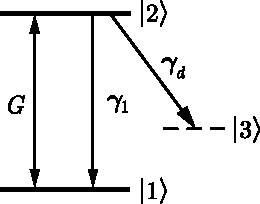
\includegraphics[width=4cm]{fig}
%  \caption{\label{f:fig}%
%  Подпись к рисунку.
%  }
%\end{figure}

%\begin{wrapfigure}{r}{0.35\textwidth}
%\centering
%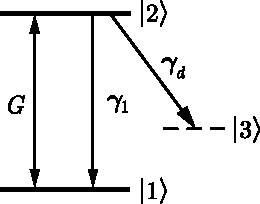
\includegraphics[width=4cm]{fig}
%\caption{\label{f:ff}%
%Рисунок <<в оборку>>.
%}
%\end{wrapfigure}

%Если разность энергий электронно-дырочных уровней $E_2 - E_1$ близка к энергии продольного оптического фонона $\hbar\Omega_{\mathrm{LO}}$, то в разложении волновых функций полного гамильтониана можно ограничиться нулевым приближением для всех состояний, за исключением близких по значению к $E_2$.
%Волновые функции последних представляют собой следующие комбинации вырожденных состояний\footnote{Текст сноски}.

%Ссылка на таблицу~\ref{t:InPSiO2}.
%\begin{table}[!ht]
%  \centering
%  \caption{Пример таблицы}\label{t:InPSiO2}
%  \begin{tabular}{l|ccc}
%    \hline\hline
%    & \quad$\lambda \cdot 10^{-11}$,~$\text{дин}\cdot\text{см}^{-2}$
%    & \quad$\mu \cdot 10^{-11}$,~$\text{дин}\cdot\text{см}^{-2}$
%    & \quad$\rho$, $\text{г}\cdot\text{см}^{-3}$ \\
%    \hline
%    InP       & 3.82 & 1.69 & 4.14 \\
%    SiO$_{2}$ & 1.57 & 3.11 & 2.2  \\
%    \hline\hline
%  \end{tabular}
%\end{table}

%\begin{figure}[!ht]
%  \centering
%  \begin{minipage}{5cm}
%    \centering
%    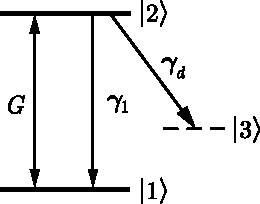
\includegraphics[width=4cm]{fig}
%    \caption{Рисунок с отдельным названием}
%  \end{minipage}
%  \quad
%  \begin{minipage}{5cm}
%    \centering
%    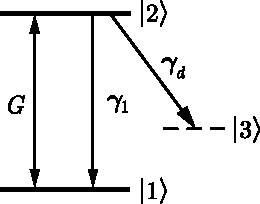
\includegraphics[width=4cm]{fig}
%    \caption{Рисунок с отдельным названием}
%  \end{minipage}
%  \quad
%  \begin{minipage}{5cm}
%    \centering
%    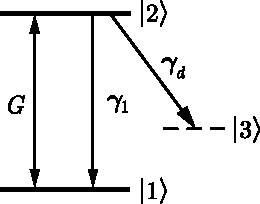
\includegraphics[width=4cm]{fig}
%    \caption{Рисунок с отдельным названием}
%  \end{minipage}
%\end{figure}

%\begin{figure}[!ht]
%  \centering
%  \begin{minipage}{5cm}
%    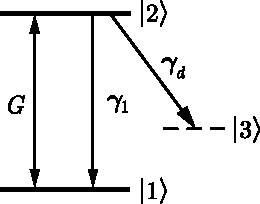
\includegraphics[width=4cm]{fig}
%  \end{minipage}
%  \begin{minipage}{5cm}
%    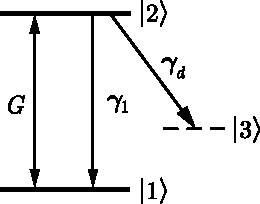
\includegraphics[width=4cm]{fig}
%  \end{minipage}
%  \caption{Рисунки с единым названием}
%\end{figure}

%Ссылка на внутренний рисунок (рис.~\ref{f:sub1}).

%\begin{figure}[!ht]
%\centering
%  \begin{minipage}{5cm}
%    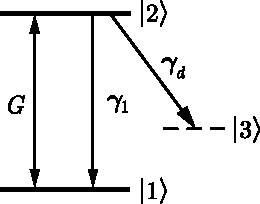
\includegraphics[width=4cm]{fig}\subcaption{}\label{f:sub1}
%  \end{minipage}
%  \begin{minipage}{5cm}
%    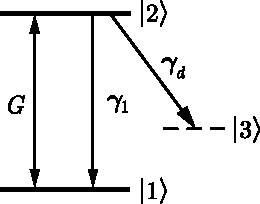
\includegraphics[width=4cm]{fig}\subcaption{}\label{f:sub2}
%  \end{minipage}
%  \begin{minipage}{5cm}
%    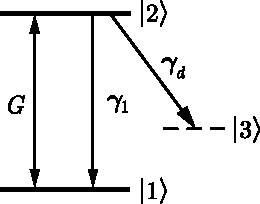
\includegraphics[width=4cm]{fig}\subcaption{}\label{f:sub3}
%  \end{minipage}
%  \caption[]{%
%  Рисунки с единым названием и подчиненной нумерацией:
%    \subref{f:sub1} ссылка 1,
%    \subref{f:sub2} ссылка 2,
%
%    \subref{f:sub3} ссылка 3.
%  }
%\end{figure}

%\subsection{Название подсекции}
%Текст подсекции
%\subsubsection{Название под-подсекции}
%Текст под-подсекции
%\paragraph{Название параграфа.}
%Текст параграфа
%\subparagraph{Название подпараграфа.}
%Текст подпараграфа

%Нумеруемый список:
%\begin{enumerate}
%  \item Первый уровень вложенности.
%  \begin{enumerate}
%    \item Второй уровень вложенности.
%    \begin{enumerate}
%      \item Третий уровень вложенности.
%    \end{enumerate}
%  \end{enumerate}
%\end{enumerate}

%Демонстрация полностью настраиваемых окружений типа <<теорема>>.

%\newtheorem{theorem}{Теорема}[chapter]
%\def\theoremstyle{}
%\def\postthetheorem{:}

%\newtheorem{lemm}{Лемма}[chapter]
%\def\thelemmstyle{\bfseries}
%\def\oparglemmstyle{}
%\def\lemmstyle{}
%\def\preoparglemm{(}
%\def\postoparglemm{):}

%\newtheorem{remark}{Примечание}[chapter]
%\def\remarkstyle{\itshape}
%\def\theremarkstyle{}
%\def\posttheremark{:}

%\begin{lemm}[Шура]
%Квадратная матрица, коммутирующая со всеми матрицами неприводимого представления, кратна единичной.
%\end{lemm}

%\begin{theorem}
%Гомоморфный образ группы изоморфен фактор-группе по ядру гомоморфизма.
%\end{theorem}

%\begin{remark}
%Текст примечания.
%\end{remark}
